\documentclass[10pt]{beamer}
\usepackage{graphicx}
\usepackage{lmodern}
\usepackage{import}

% Changes beamer so it'll look for .sty files in the sty/ directory
\makeatletter
    \def\beamer@calltheme#1#2#3{%
        \def\beamer@themelist{#2}
        \@for\beamer@themename:=\beamer@themelist\do
        {\input{sty/#3\beamer@themename.sty}}}

\usetheme{metropolis}

% Without this, warning are shown for using pdf_tex files
\pdfsuppresswarningpagegroup=1

% Don't show nav buttons
\beamertemplatenavigationsymbolsempty

\title[Project]{COSC3000: Data visualisation project}
\subtitle{War visualised}
\author{John Owen}
\titlegraphic{
    \vspace{19em}
    \centering
    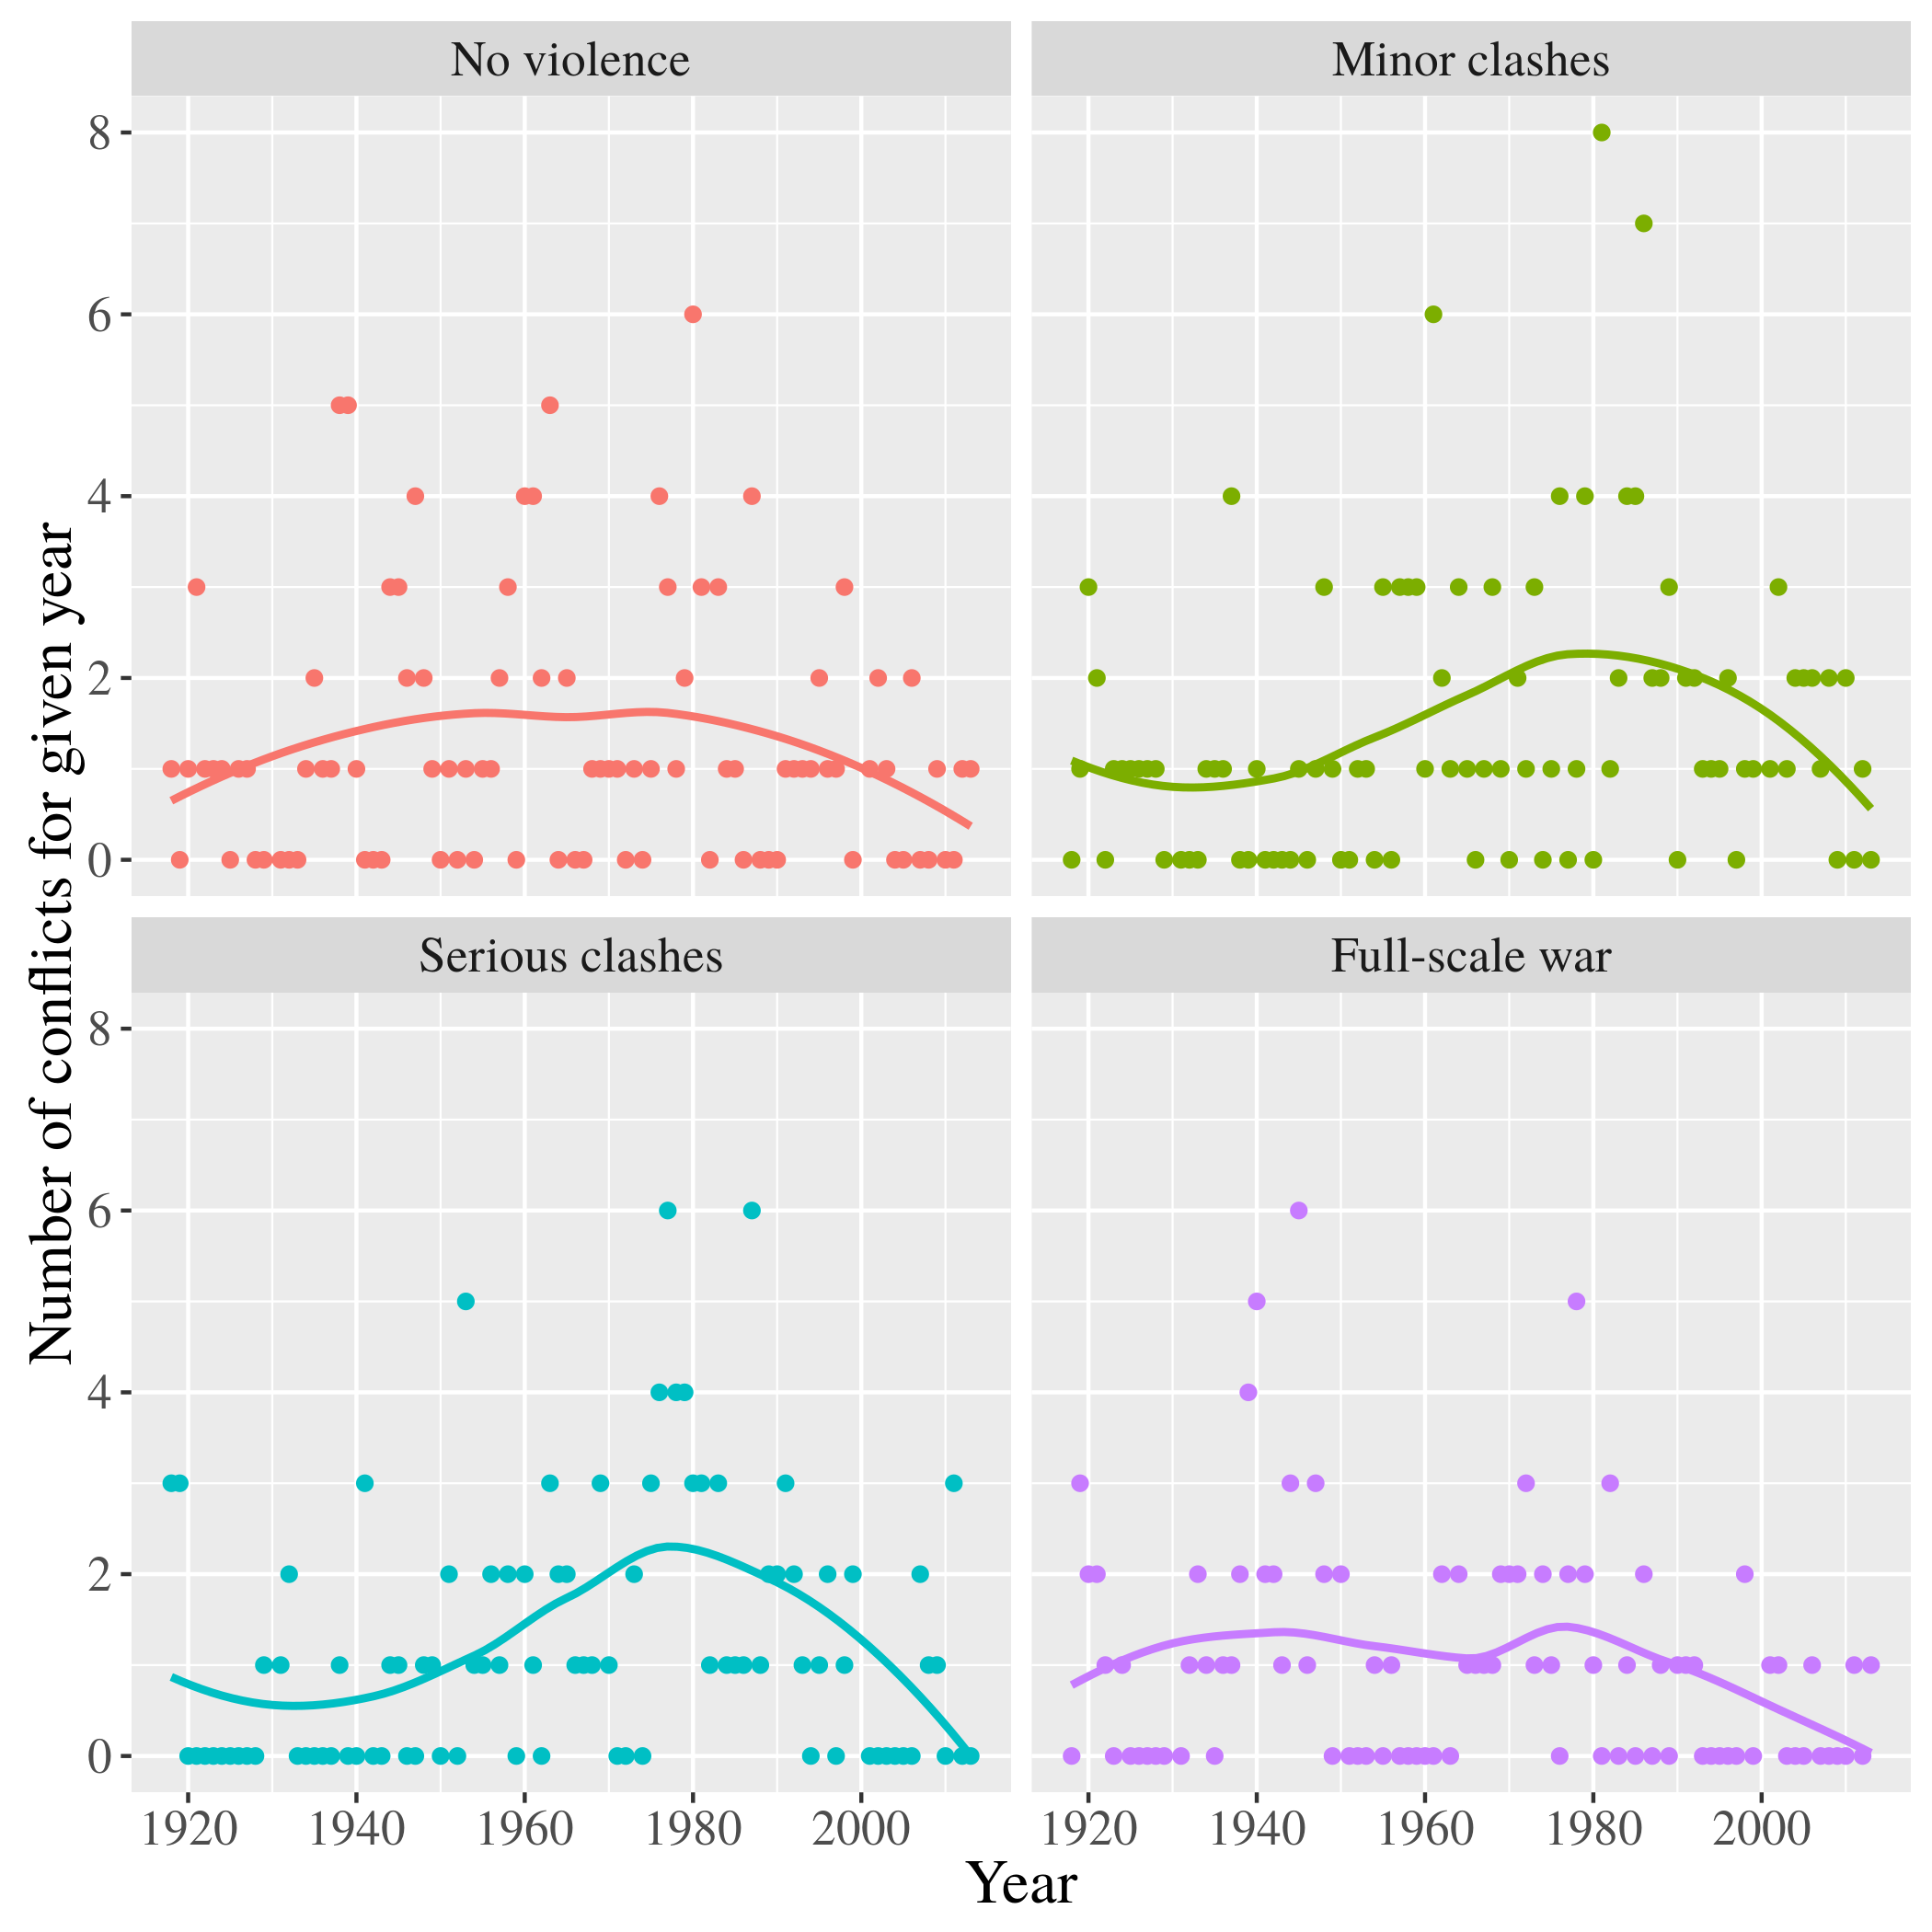
\includegraphics[width=\textwidth,height=0.27\textheight,keepaspectratio]{tmp/war_over_time.pdf}
    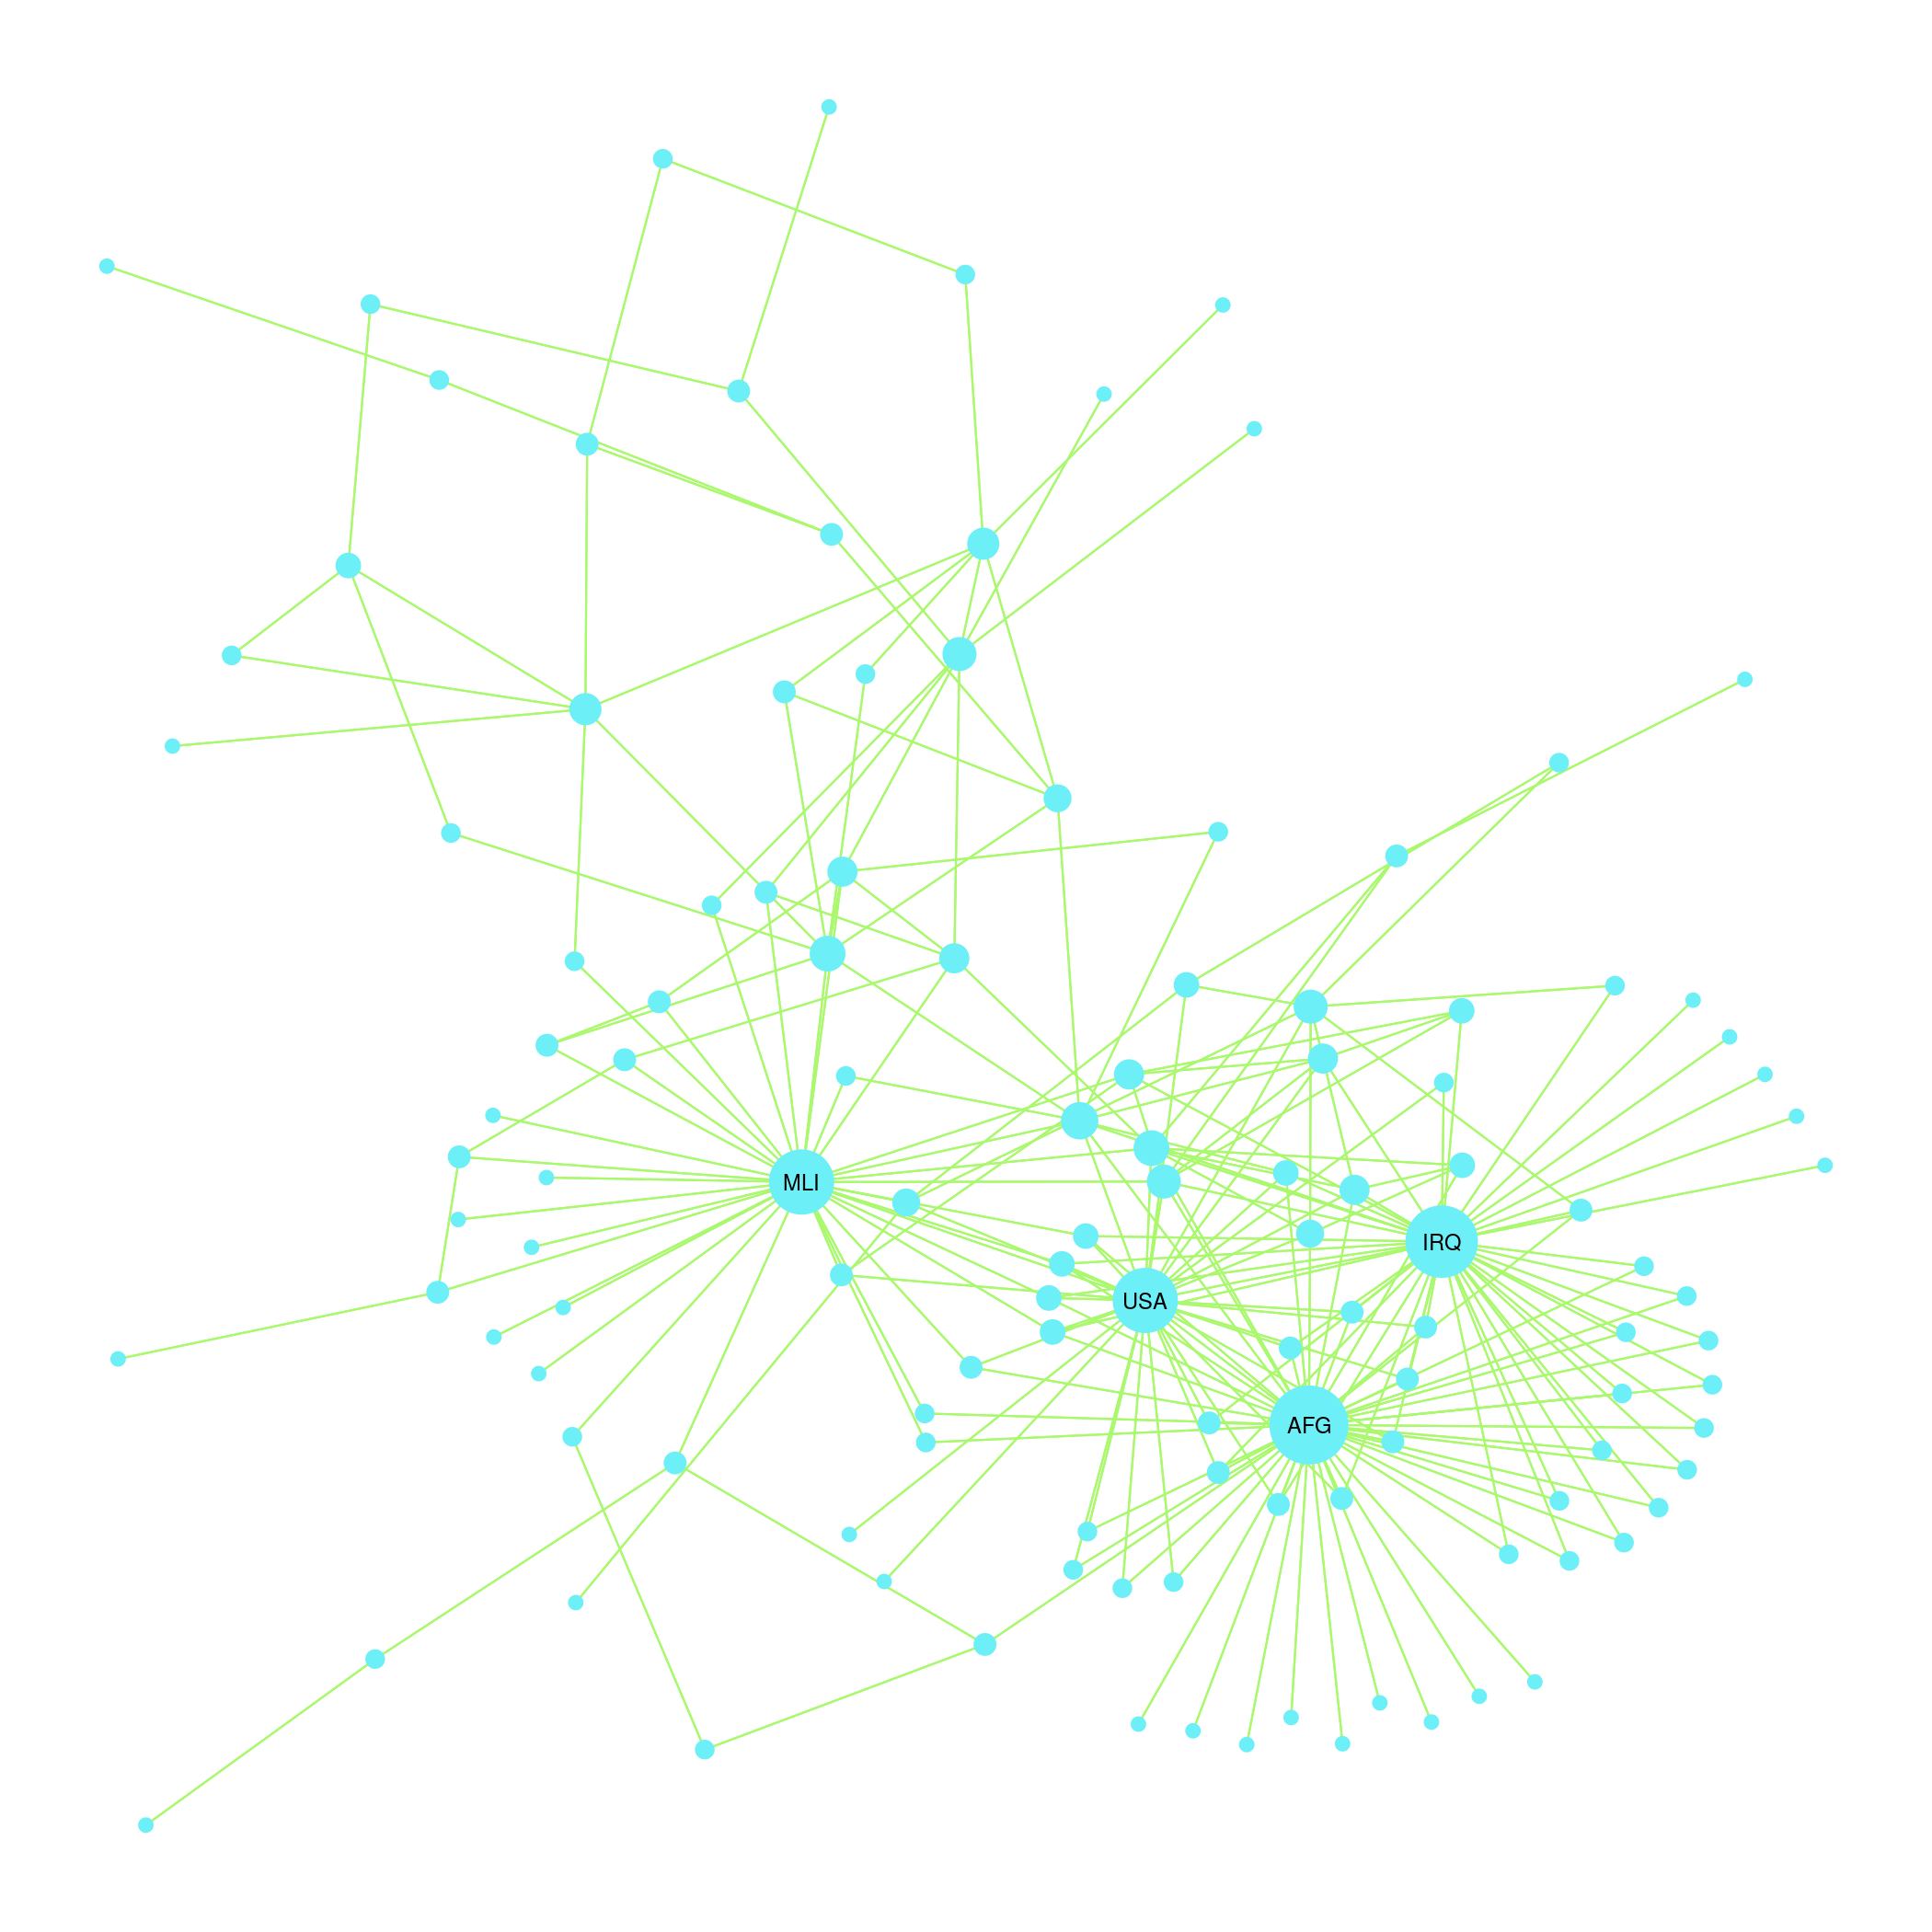
\includegraphics[width=\textwidth,height=0.27\textheight,keepaspectratio]{tmp/ally_network.pdf}
    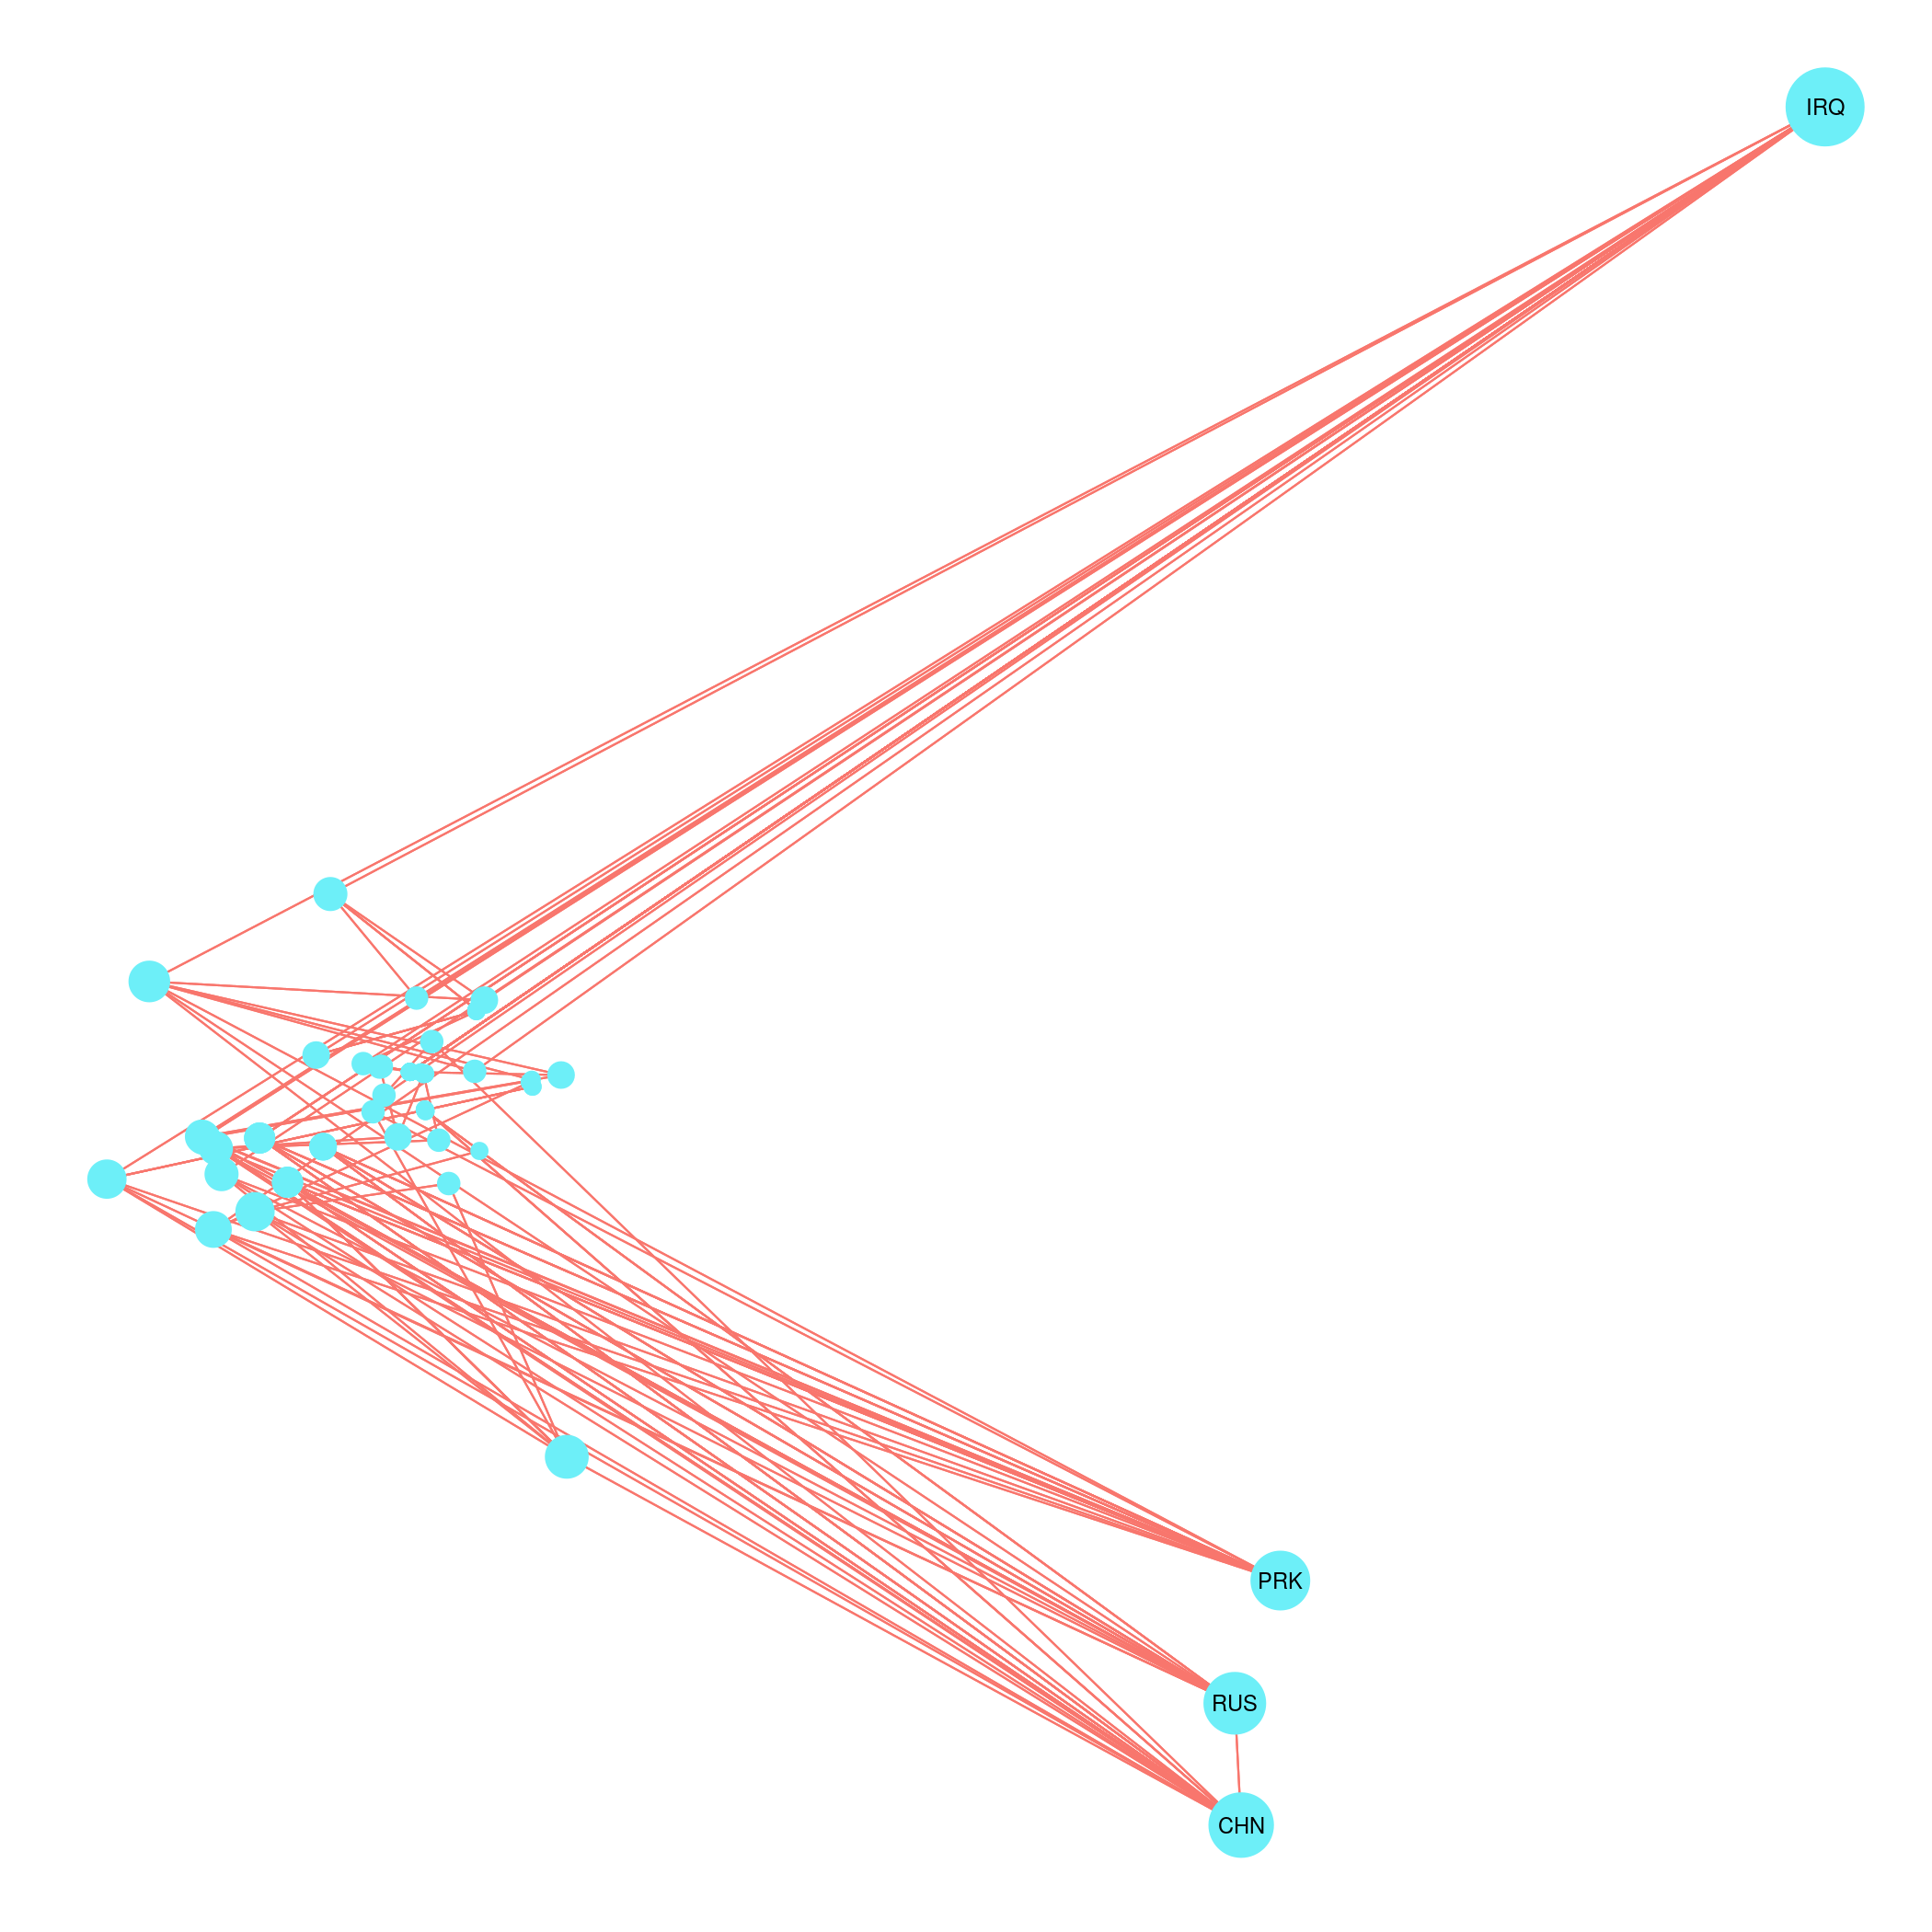
\includegraphics[width=\textwidth,height=0.27\textheight,keepaspectratio]{tmp/enemy_network.pdf}
    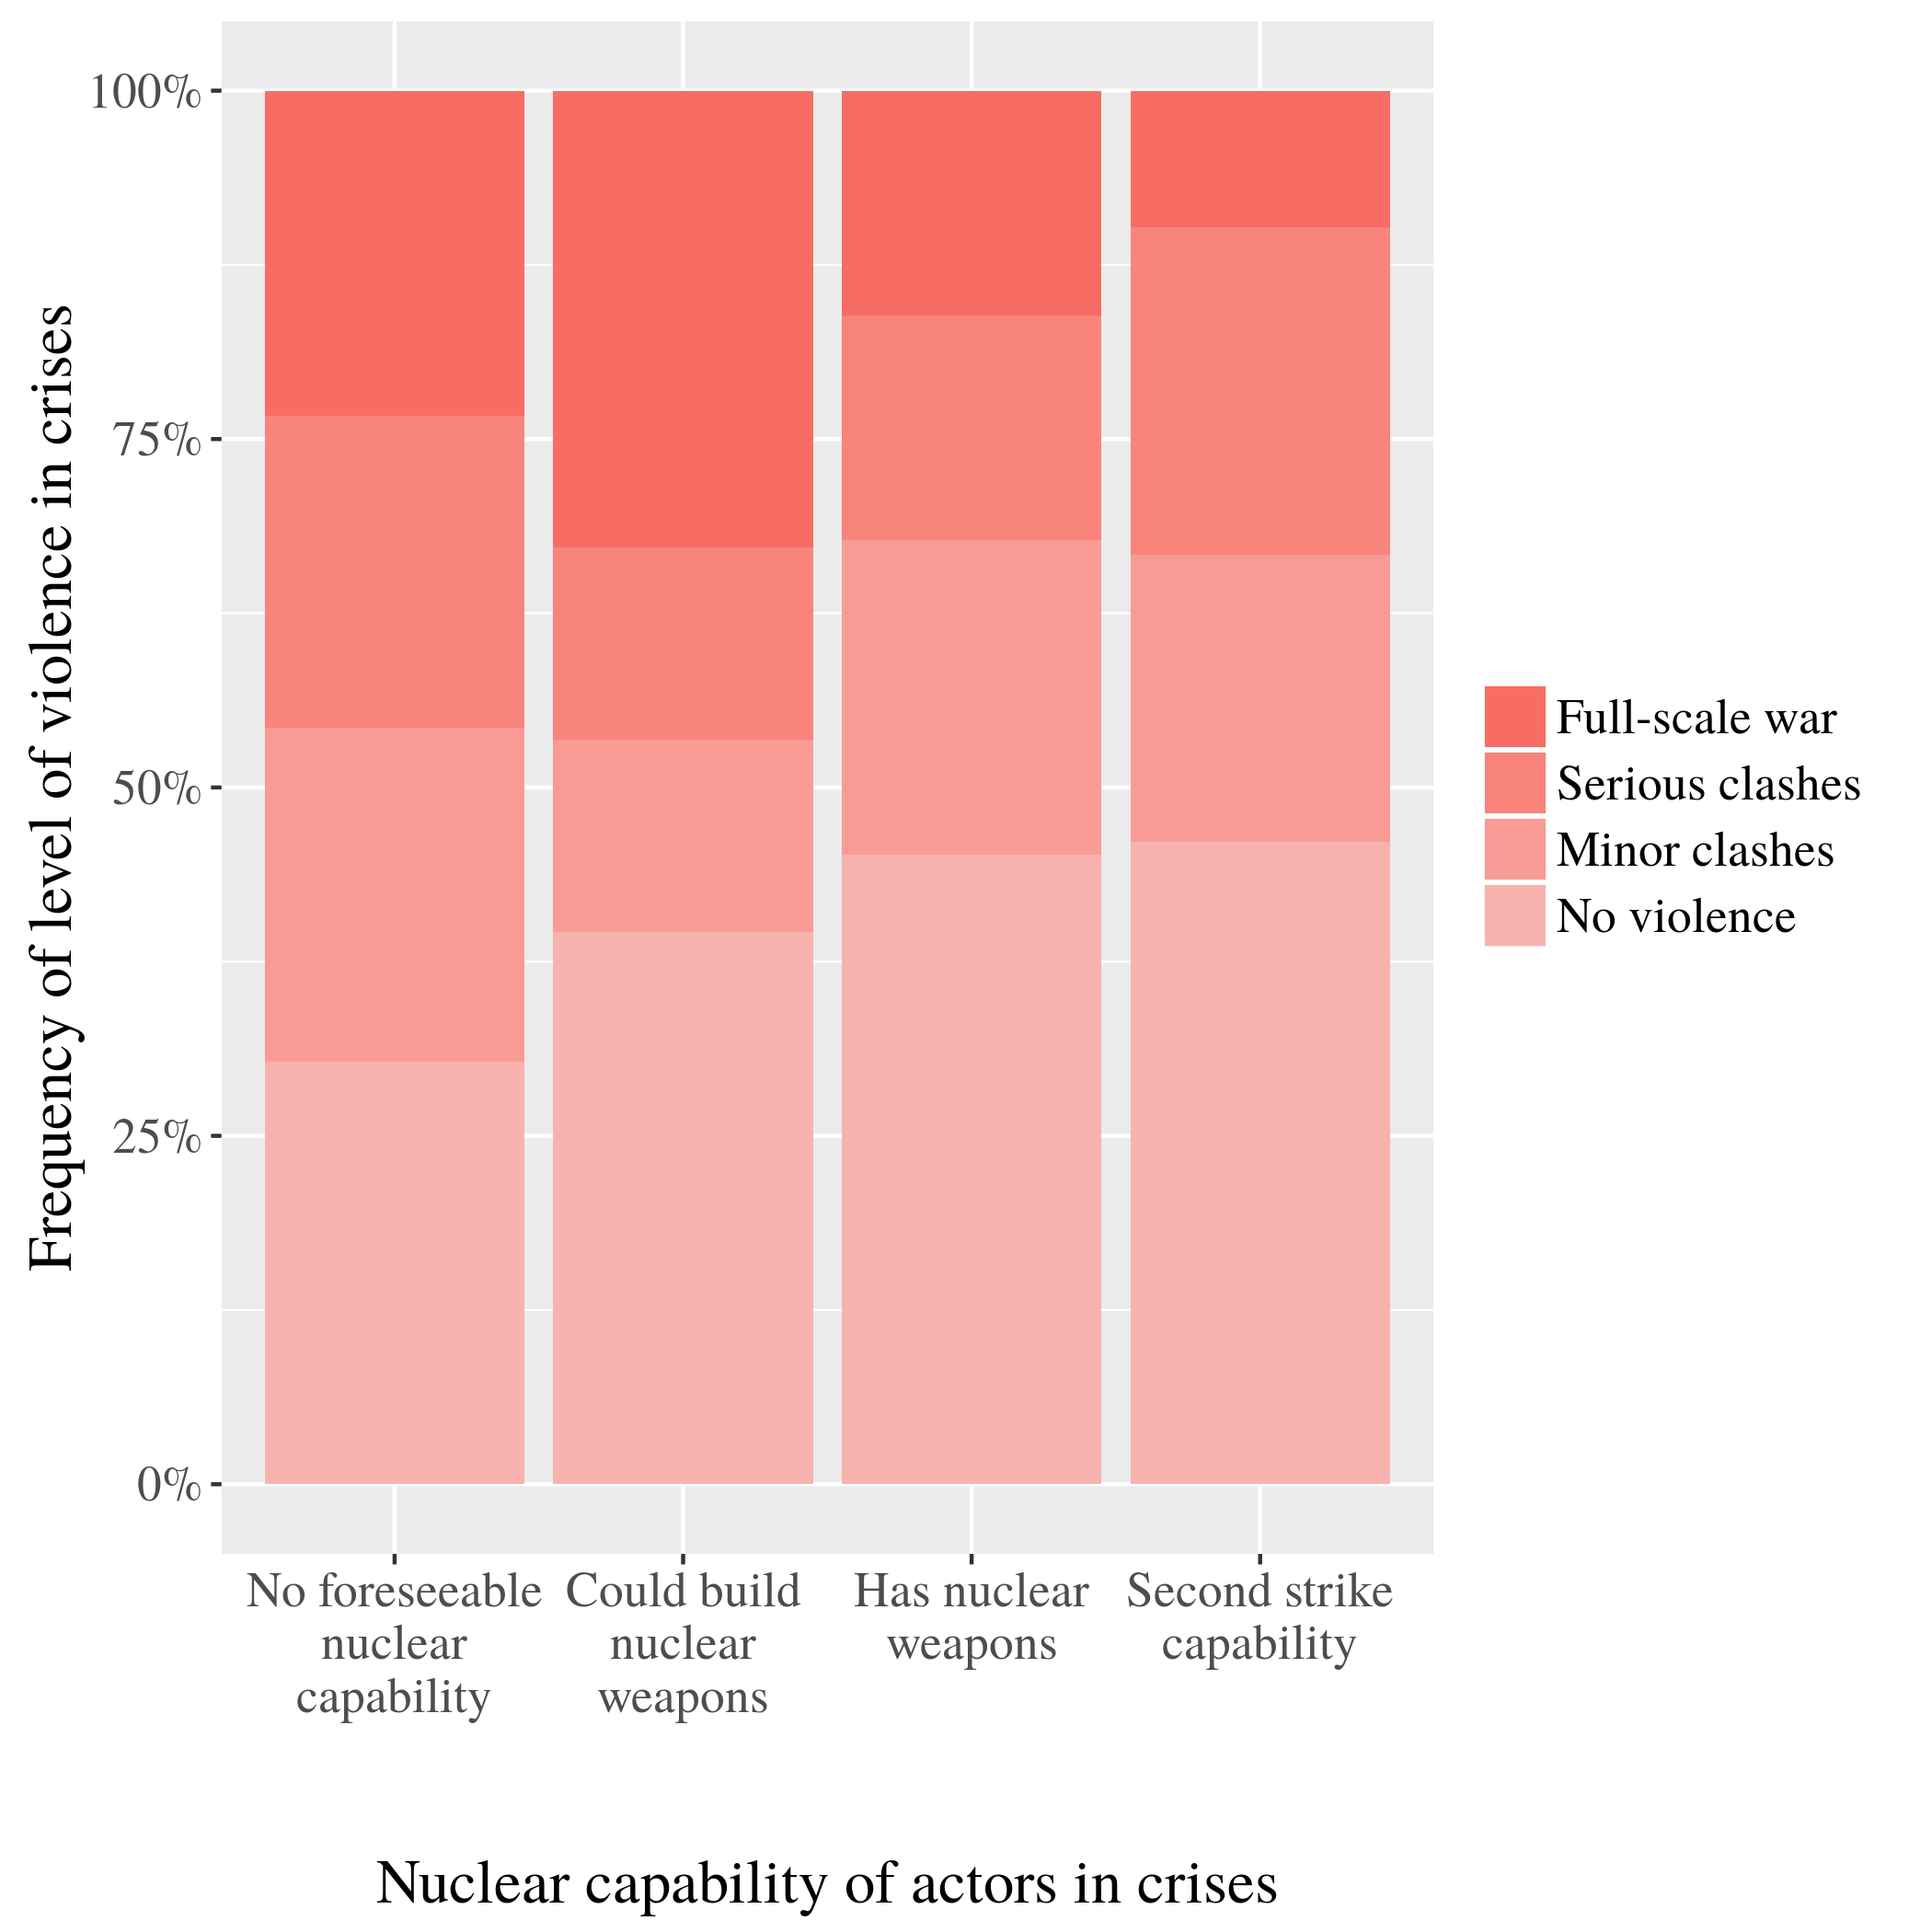
\includegraphics[width=\textwidth,height=0.27\textheight,keepaspectratio]{tmp/nuclear_compared_with_violence.pdf}
}

\newcommand\fullsizeimage[1]{
    \begin{center}
        \includegraphics[width=\textwidth,height=0.8\textheight,keepaspectratio]{#1}
    \end{center}
}

\newcommand\includepdftex[2]{
    \def\svgwidth{#1}
    \import{tmp/}{#2}
}

\begin{document}

\frame{
    \vspace{-4em}
    \titlepage
}

\frame{
    \frametitle{Project aim}
    \begin{columns}
        \column{.6\textwidth}
        \begin{itemize}
            \item Find interesting things about war
                \begin{itemize}
                    \item How war changes over time
                    \item Main players
                    \item Nukes
                \end{itemize}
            \item UCDP/PRIO Armed Conflict dataset
            \item International Crisis Behavior Project dataset
        \end{itemize}
        \column{.4\textwidth}
        \centering
        \includepdftex{\columnwidth}{tmp/ucdp-prio.pdf_tex}
        \\~\\
        
\includegraphics[width=\columnwidth]{img/icb.png} 
    \end{columns}
}

\frame{
    \frametitle{Motivation}
    \begin{itemize}
        \item Understanding war is important for politicians and voters
        \item Long articles are time consuming and don't allow for comparison
        \item Graphs provide are an alternative
    \end{itemize}
}

\frame{
    \frametitle{Datasets used}
    \begin{columns}
        \column{.6\textwidth}
        \begin{block}{UCDP/PRIO Armed Conflict dataset}
            A list of conflicts
            \begin{itemize}
                \item When and where was the conflict
                \item Who was on what side (conflict actors)
                \item Type of conflict (civil war, international war, other
                    possibilities)
                \item Intensity of conflict
            \end{itemize}
        \end{block}

        \begin{block}{Gleditch and Ward list of states}
            Maps state IDs in the UCDP/PRIO dataset to state names \\
            (e.g, 2 $\rightarrow$ ``United States of America'').
        \end{block}
        
        \column{.4\textwidth}
        \centering
        \includepdftex{0.6\columnwidth}{tmp/ucdp.pdf_tex}
        \vspace{2em}
        \includepdftex{0.8\columnwidth}{tmp/prio.pdf_tex}
    \end{columns}
}

\frame{
    \frametitle{Datasets used}
    \begin{columns}
        \column{.6\textwidth}
        \begin{block}{International Crisis Behavior Project dataset}
            A list of military security crises
            \begin{itemize}
                \item What was the cause of the crises
                \item How much did the opposing sides communicate
                \item How did the actors manage the crisis (economic sanctions,
                    violence, etc)
                \item Global organizations like the UN
                \item Nuclear weapon capability
            \end{itemize}
        \end{block}
        \column{.4\textwidth}
        \centering
        
\includegraphics[width=\columnwidth]{img/icb.png}
    \end{columns}
}

\frame{
    \frametitle{Method}
    \begin{columns}
        \column{0.6\textwidth}
        I used the R language to create the graphics.
        \begin{block}{\texttt{main.R}}
            \begin{itemize}
                \item Load datasets from CSV files
                \item Parse numeric and vector columns
                \item Coerce data to format needed for graphing (e.g, adjacency
                    matrix, frequency table, network)
                \item Plot data with the ``ggplot2'' library
            \end{itemize}
        \end{block}
        \column{0.4\textwidth}
        \includepdftex{\columnwidth}{tmp/r.pdf_tex}
    \end{columns}
}

\frame{
    \frametitle{Results}
    \framesubtitle{War over time}
    \fullsizeimage{tmp/war_over_time.pdf}
}

\frame{
    \frametitle{Results}
    \framesubtitle{War over time}
    \begin{columns}
        \column{.5\textwidth}
        Conflicts peak in the late 70's and then drop drastically
        \begin{itemize}
            \item End of cold war
            \item Collapse of soviet union
        \end{itemize}
        \column{0.5\textwidth}
        \fullsizeimage{tmp/war_over_time.pdf}
    \end{columns}
}

\frame{
    \frametitle{Results}
    \framesubtitle{Nuclear weapon capability vs crisis violence}
    \fullsizeimage{tmp/nuclear_compared_with_violence.pdf}
}

\frame{
    \frametitle{Results}
    \framesubtitle{Nuclear weapon capability vs crisis violence}
    \begin{columns}
        \column{.5\textwidth}
        \begin{description}
            \item[No foreseeable nuclear capability] Couldn't build nukes
                within 5 years
            \item[Foreseeable nuclear capability] Could build nukes within
                5 years
            \item[Possession of nuclear weapons] Has nukes
            \item[With second strike capability] If attacked with nuclear
                weapons, could still retaliate
        \end{description}
        \column{.5\textwidth}
        \fullsizeimage{tmp/nuclear_compared_with_violence.pdf}
    \end{columns}
}

\frame{
    \frametitle{Results}
    \framesubtitle{Nuclear weapon capability vs crisis violence}
    \begin{columns}
        \column{.5\textwidth}
        \begin{itemize}
            \item Higher nuclear capability associated with a higher
                frequency of non-violent crises (i.e, events that
                \textit{could} have become violent but didn't)
            \item Why?...
        \end{itemize}
        \column{.5\textwidth}
        \fullsizeimage{tmp/nuclear_compared_with_violence.pdf}
    \end{columns}
}

\frame{
    \frametitle{Results}
    \framesubtitle{Nuclear weapon capability vs crisis violence}
    \begin{columns}
        \column{.5\textwidth}
        Commonly held hypothesis:
        \begin{itemize}
            \item Nukes decrease likelihood of conflict b.c governments
                are afraid of a mutually destructive nuclear war, as seen
                in the Cold War
            \item However, beyond a certain level, bolstering a nuclear
                arsenal doesn't decrease conflicts
        \end{itemize}
        If this hypothesis were true, this would be the expected result
        \column{.5\textwidth}
        \fullsizeimage{tmp/nuclear_compared_with_violence.pdf}
    \end{columns}
}

\frame{
    \frametitle{Results}
    \framesubtitle{Network of allies}
    \fullsizeimage{tmp/ally_network.pdf}
}

\frame{
    \frametitle{Results}
    \framesubtitle{Network of allies}
    \begin{columns}
        \column{.5\textwidth}
        \begin{itemize}
            \item \onslide<1->{Nodes are countries}
            \item \onslide<1->{Edges are between states that have fought on the same side}
            \item \onslide<2->{Countries that haven't fought with any
                allies aren't shown (i.e, nodes with no edges)}
            \item \onslide<3->{Four countries with many more allies than
                    other countries are labeled
                    \begin{itemize}
                        \item Mali (MLI)
                        \item United States of America (USA)
                        \item Afghanistan (AFG)
                        \item Iraq (IRQ)
                    \end{itemize}}
            \item \onslide<4->{The size of each node is determined by the
                number of edges it has}
        \end{itemize}
        \column{.5\textwidth}
        \onslide<1->{\fullsizeimage{tmp/ally_network.pdf}}
    \end{columns}
}

\frame{
    \frametitle{Results}
    \framesubtitle{Network of allies}
    \begin{columns}
        \column{.5\textwidth}
        \begin{itemize}
            \item Most countries that have fought wars with allies do so
                with only a few
            \item Some countries fight with many allies (Mali, United
                States of America, Afghanistan, and Iraq)
        \end{itemize}
        \column{.5\textwidth}
        \fullsizeimage{tmp/ally_network.pdf}
    \end{columns}
}

\frame{
    \frametitle{Results}
    \framesubtitle{Network of enemies}
    \fullsizeimage{tmp/enemy_network.pdf}
}

\frame{
    \frametitle{Results}
    \framesubtitle{Network of enemies}
    \begin{columns}
        \column{.5\textwidth}
        \begin{itemize}
            \item \onslide<1->{Nodes are countries}
            \item \onslide<1->{Edges are between states that have fought
                against each other}
            \item \onslide<2->{Countries that haven't fought anyone aren't
                show}
            \item \onslide<3->{Four countries who've fought with many
                    other countries are labeled
                    \begin{enumerate}
                        \item Iraq (IRQ)
                        \item North Korea (PRK)
                        \item Russia (RUS)
                        \item China (CHN)
                    \end{enumerate}}
            \item \onslide<4->{The size of each node is determined by the
                number of edges it has}
        \end{itemize}
        \column{.5\textwidth}
        \onslide<1->{\fullsizeimage{tmp/enemy_network.pdf}}
    \end{columns}
}

\frame{
    \frametitle{Results}
    \framesubtitle{Network of enemies}
    \begin{columns}
        \column{.5\textwidth}
        \begin{itemize}
            \item Most countries that have fought wars with allies do so
                with only a few
            \item Some countries fight with many allies (Mali, United
                States of America, Afghanistan, and Iraq)
        \end{itemize}
        \column{.5\textwidth}
        \fullsizeimage{tmp/enemy_network.pdf}
    \end{columns}
}

\frame{
    \frametitle{Results}
    \framesubtitle{Network of enemies}
    \begin{columns}
        \column{.5\textwidth}
        \begin{itemize}
            \item USA doesn't have noticeably more enemies than everyone
                else
            \item Cold War: USA avoids direct conflict with Russia
            \item Fears war could cause a nuclear apocalypse
            \item Adopts indirect approach to wars, chooses to arm and
                train armies and rebel groups instead, so called ``proxy
                wars''
        \end{itemize}
        \column{.5\textwidth}
        \fullsizeimage{tmp/enemy_network.pdf}
    \end{columns}
}

\frame[plain]{
    \begin{table}[]
        \centering
        \begin{tabular}{ll}
            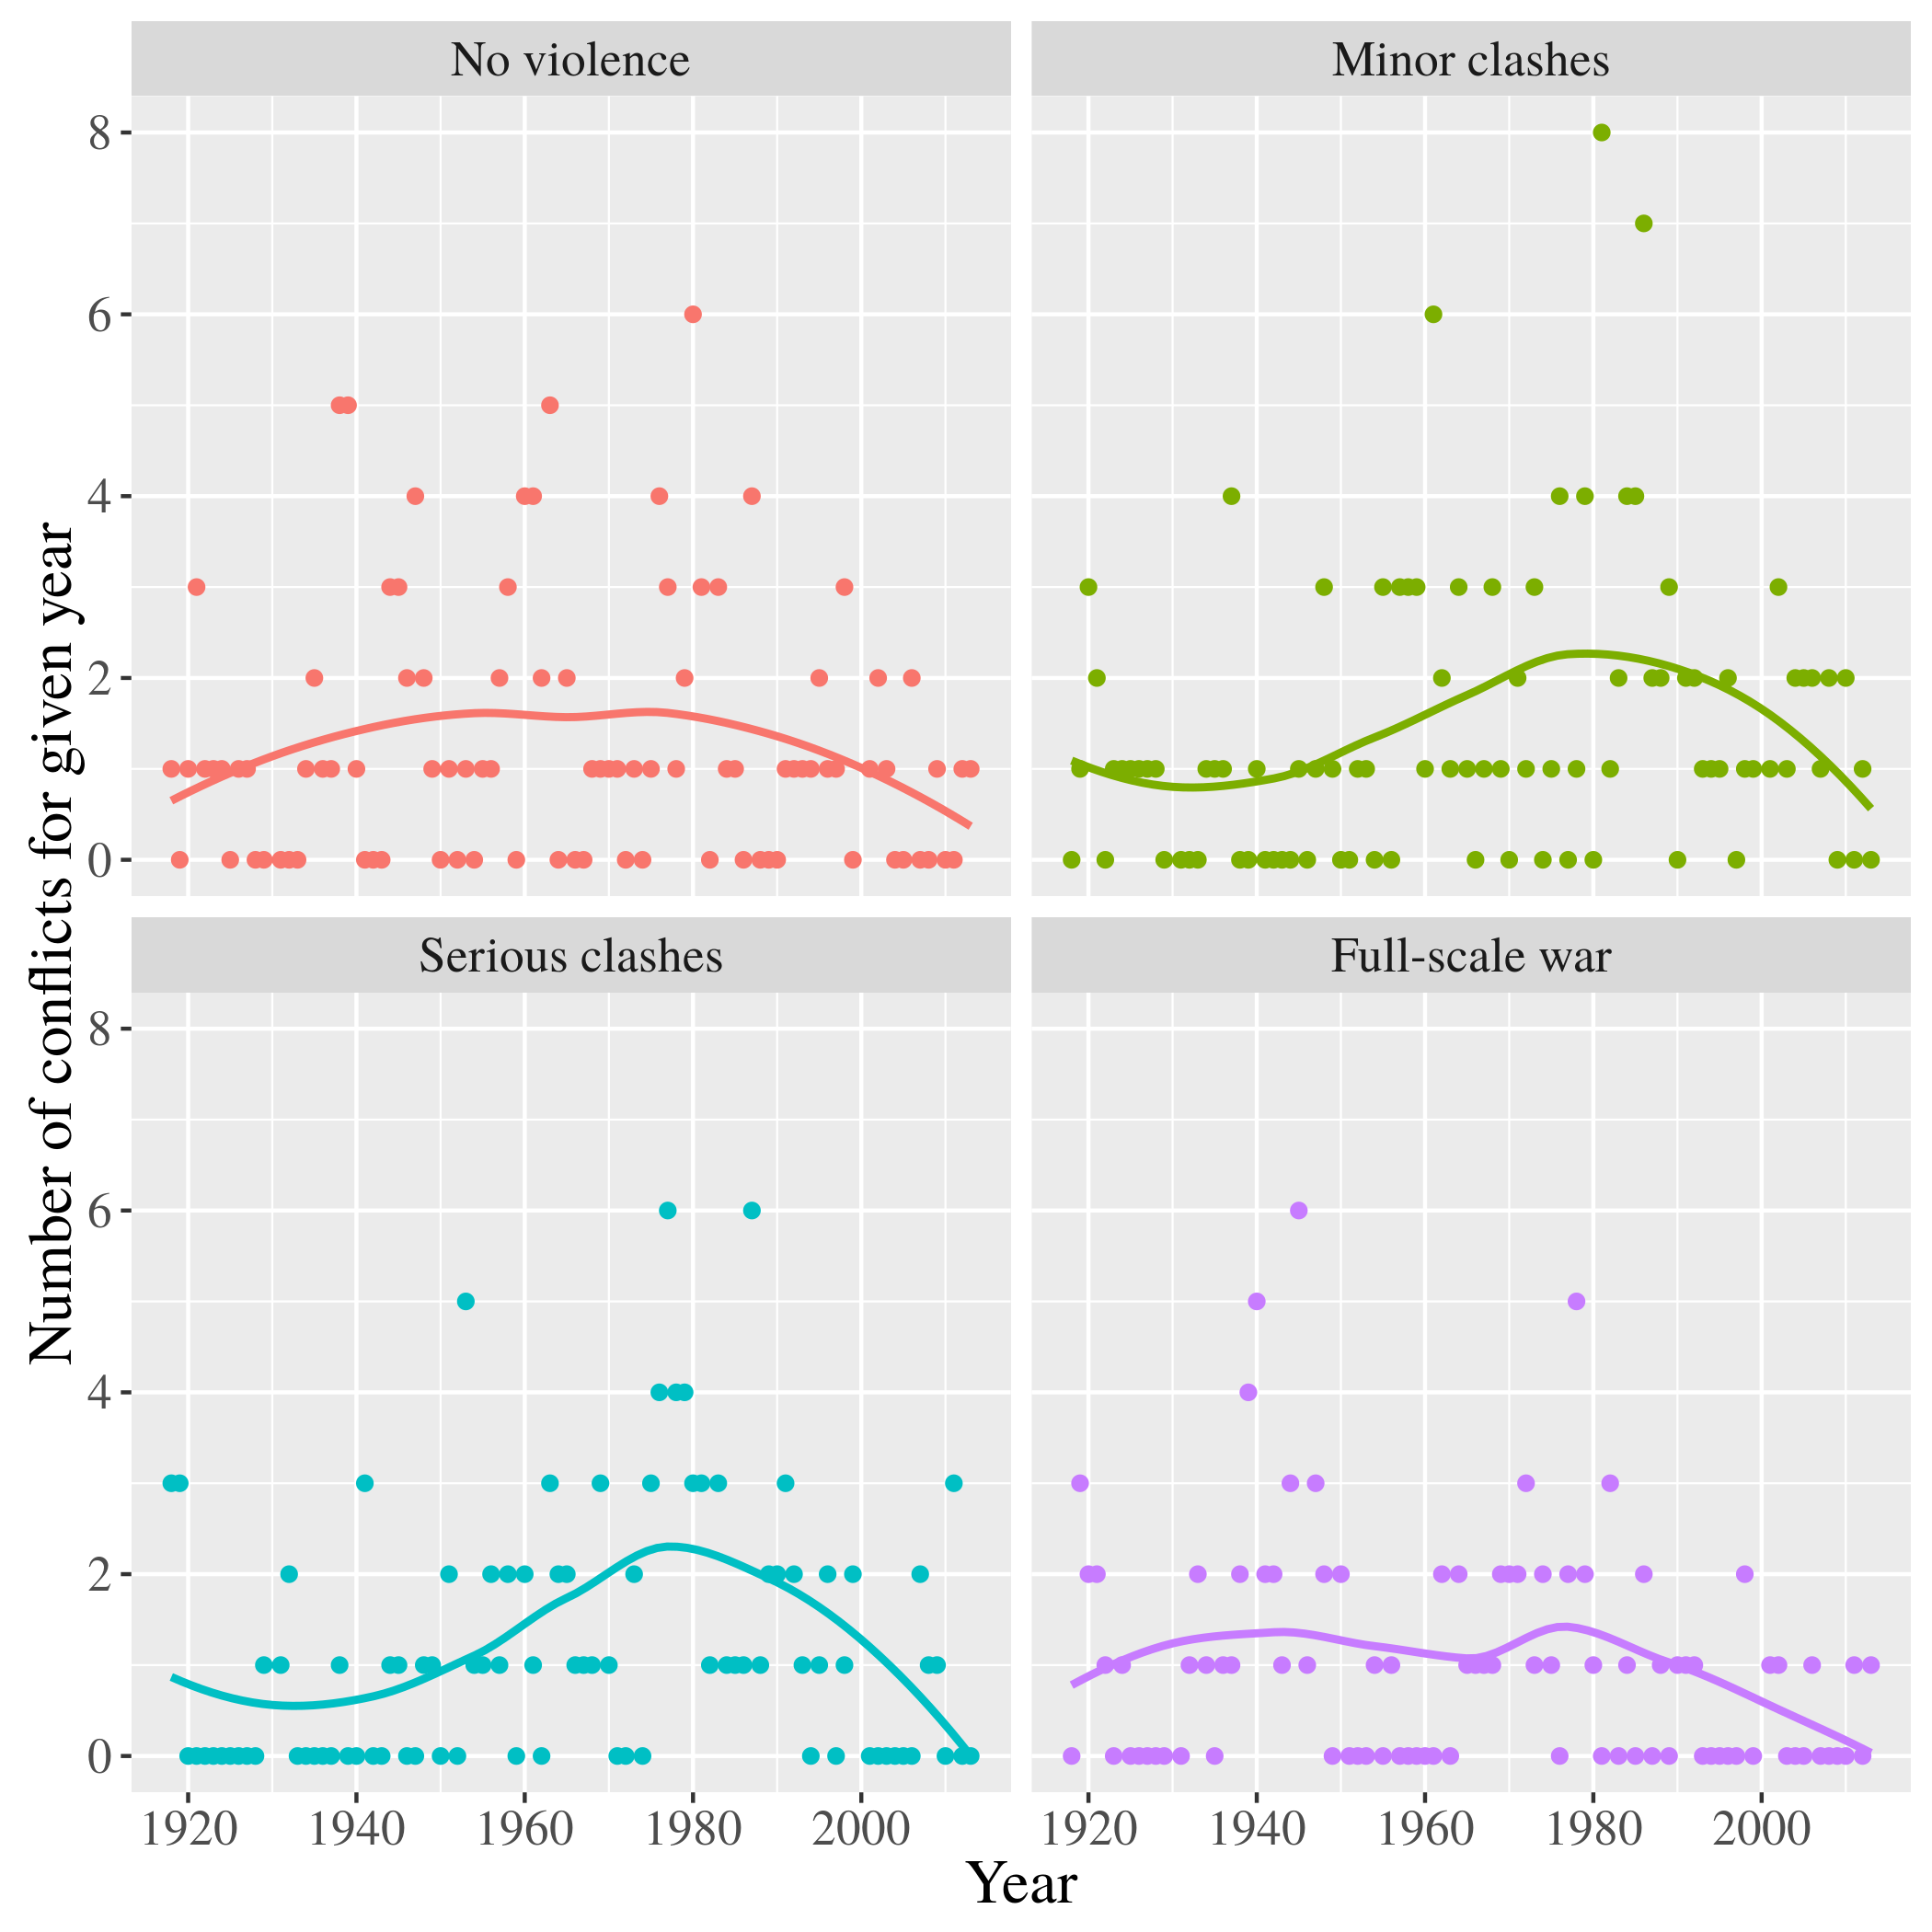
\includegraphics[width=\textwidth,height=0.47\textheight,keepaspectratio]{tmp/war_over_time.pdf} &
            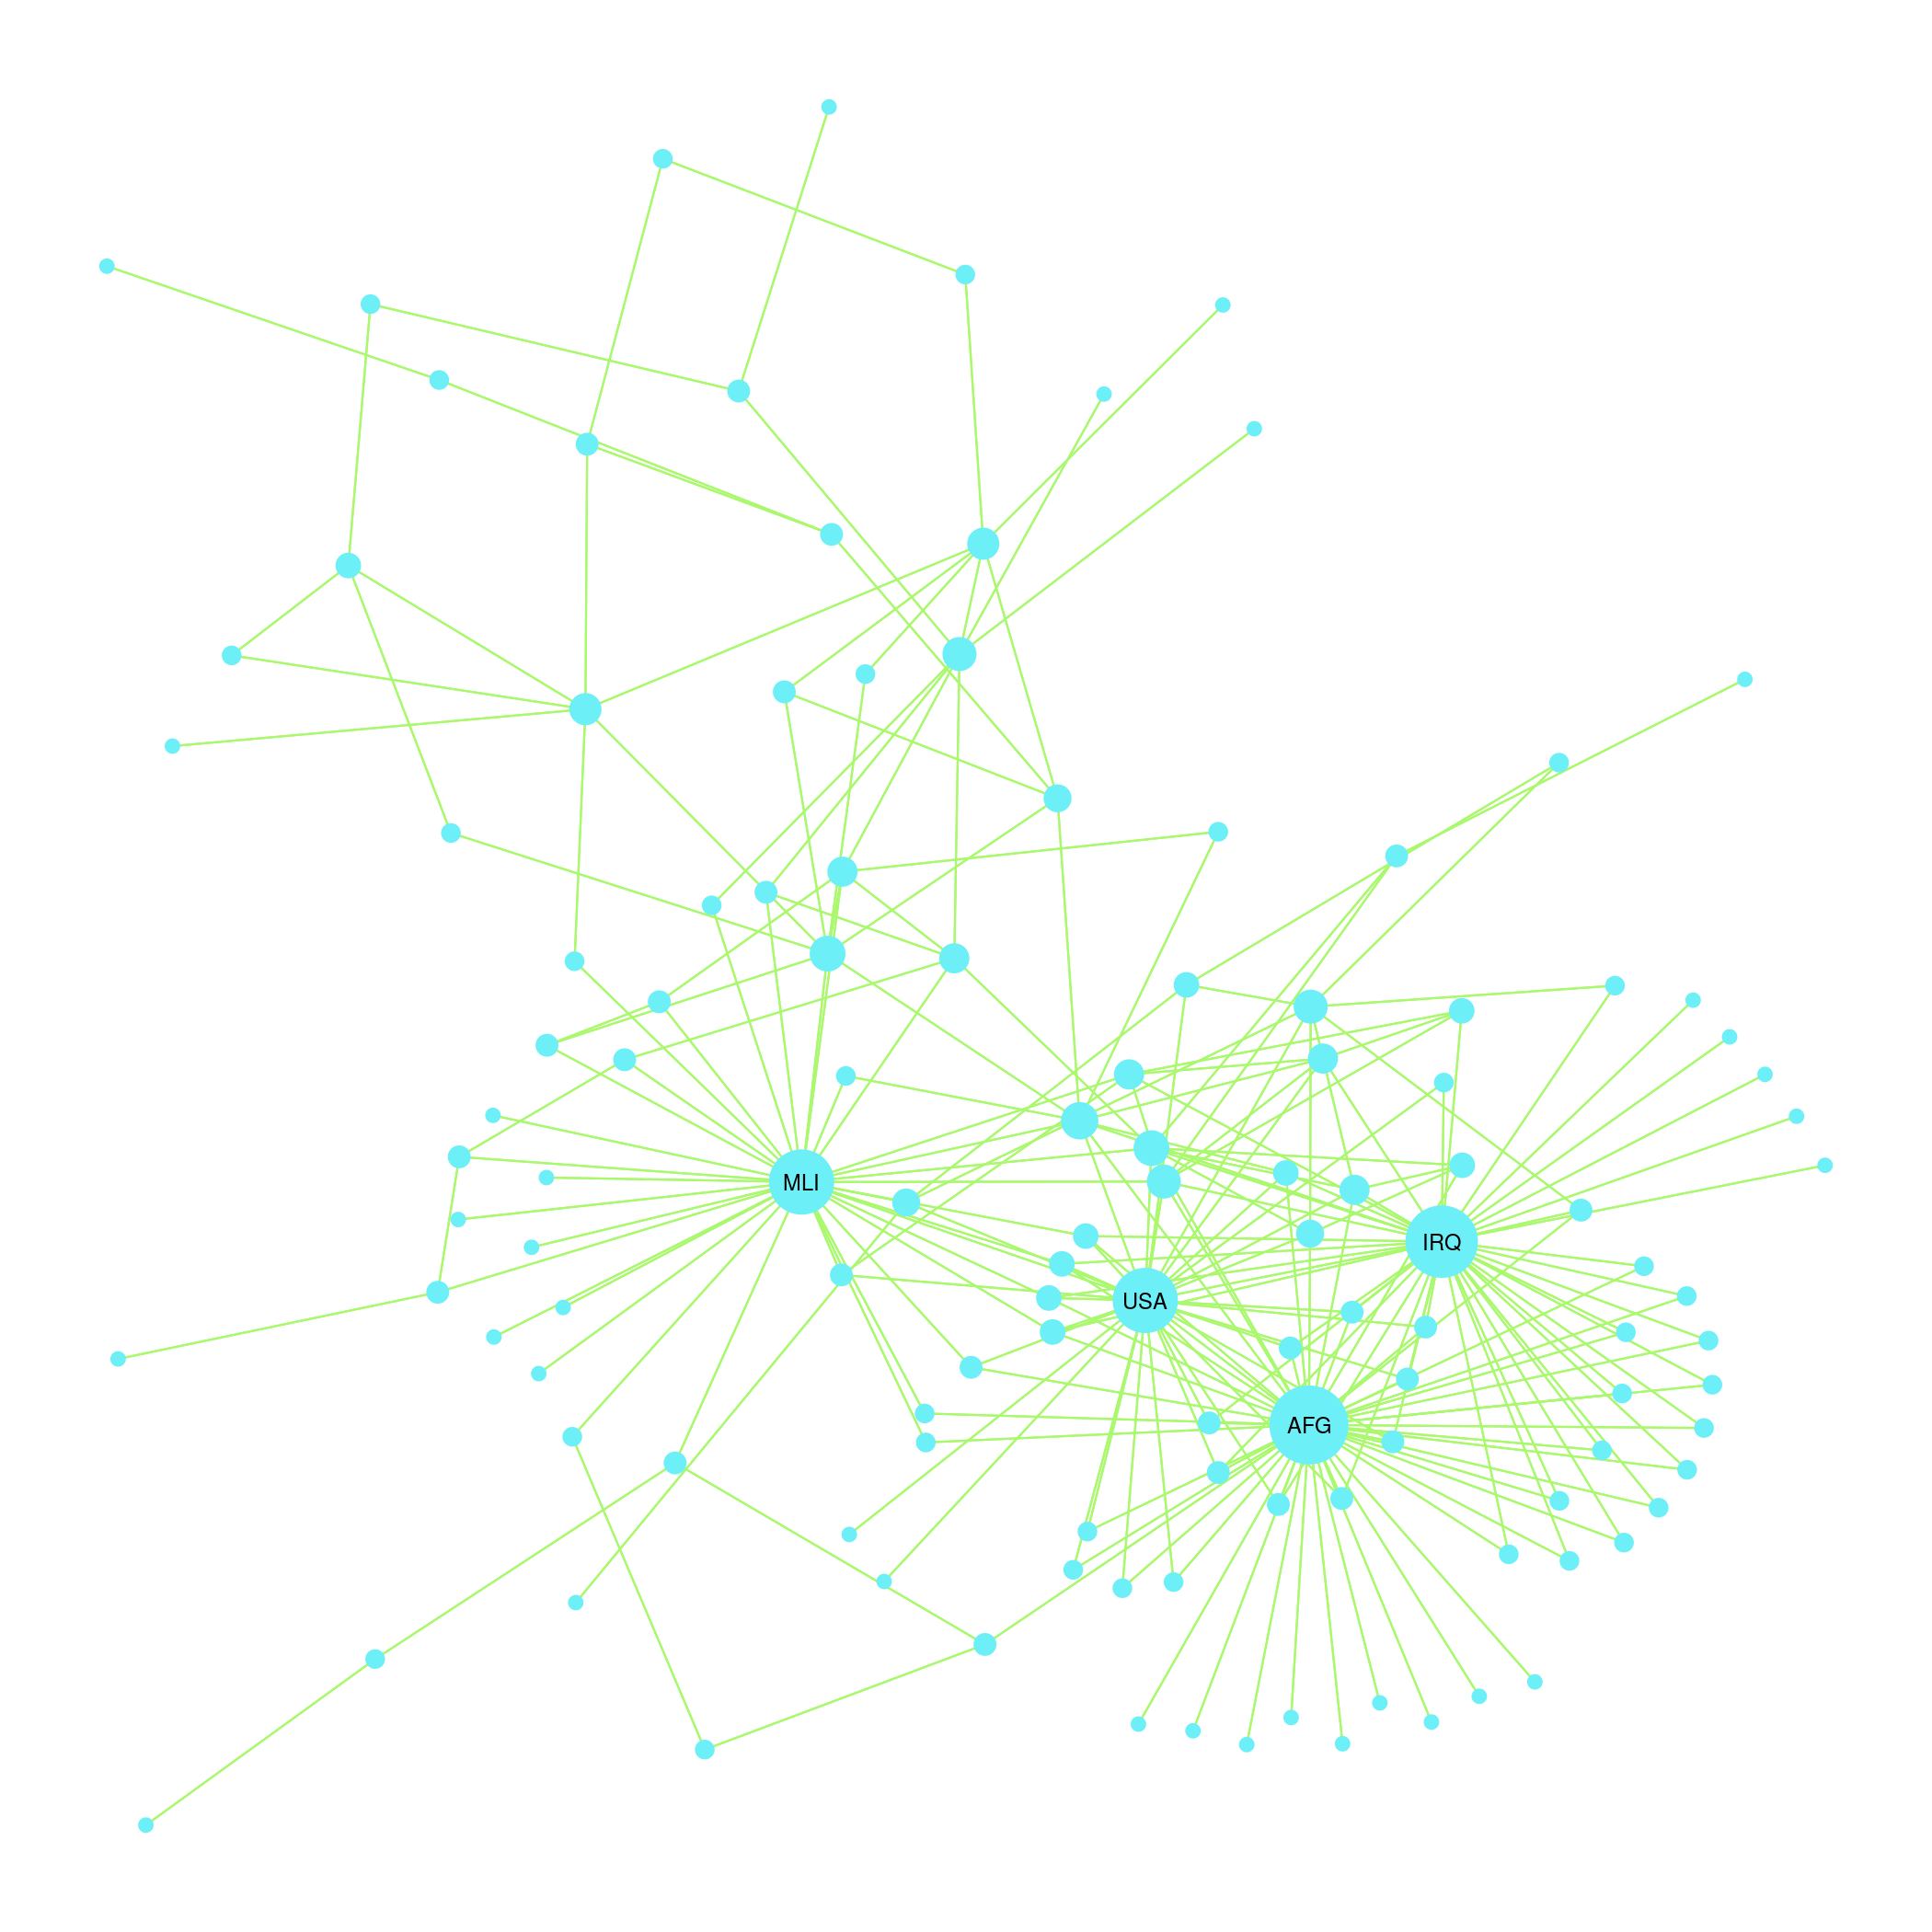
\includegraphics[width=\textwidth,height=0.47\textheight,keepaspectratio]{tmp/ally_network.pdf} \\
            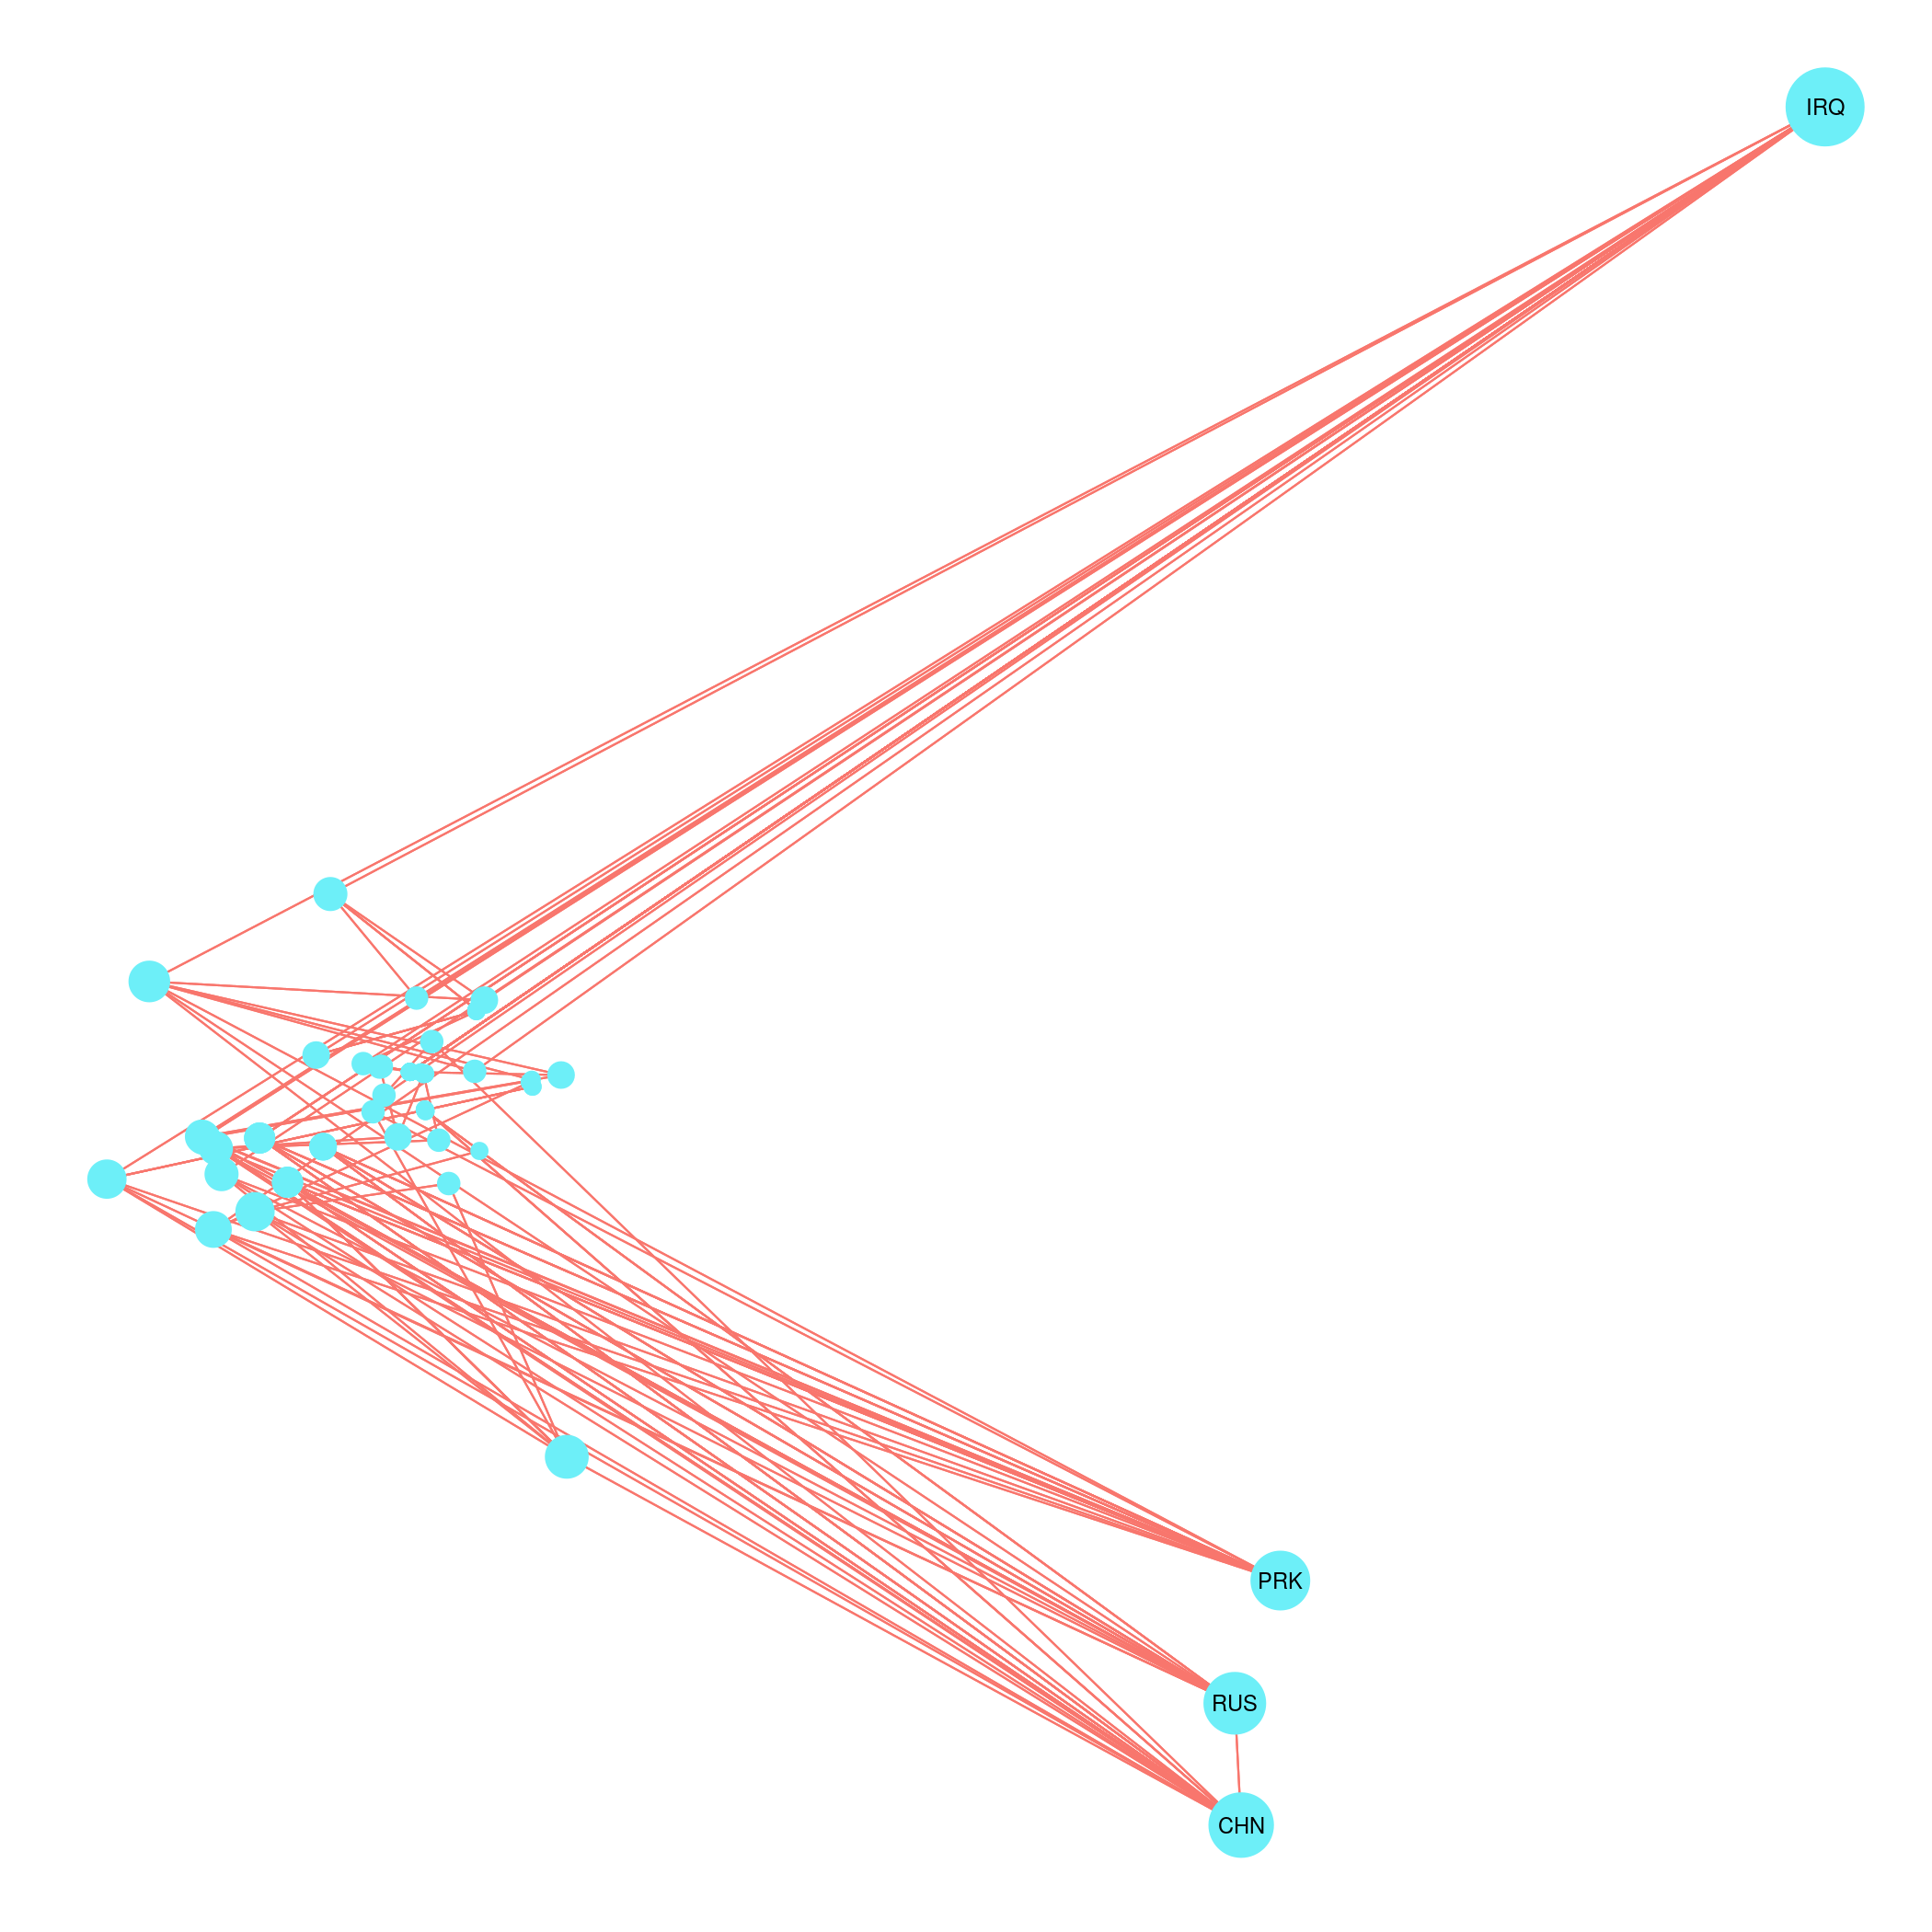
\includegraphics[width=\textwidth,height=0.47\textheight,keepaspectratio]{tmp/enemy_network.pdf} &
            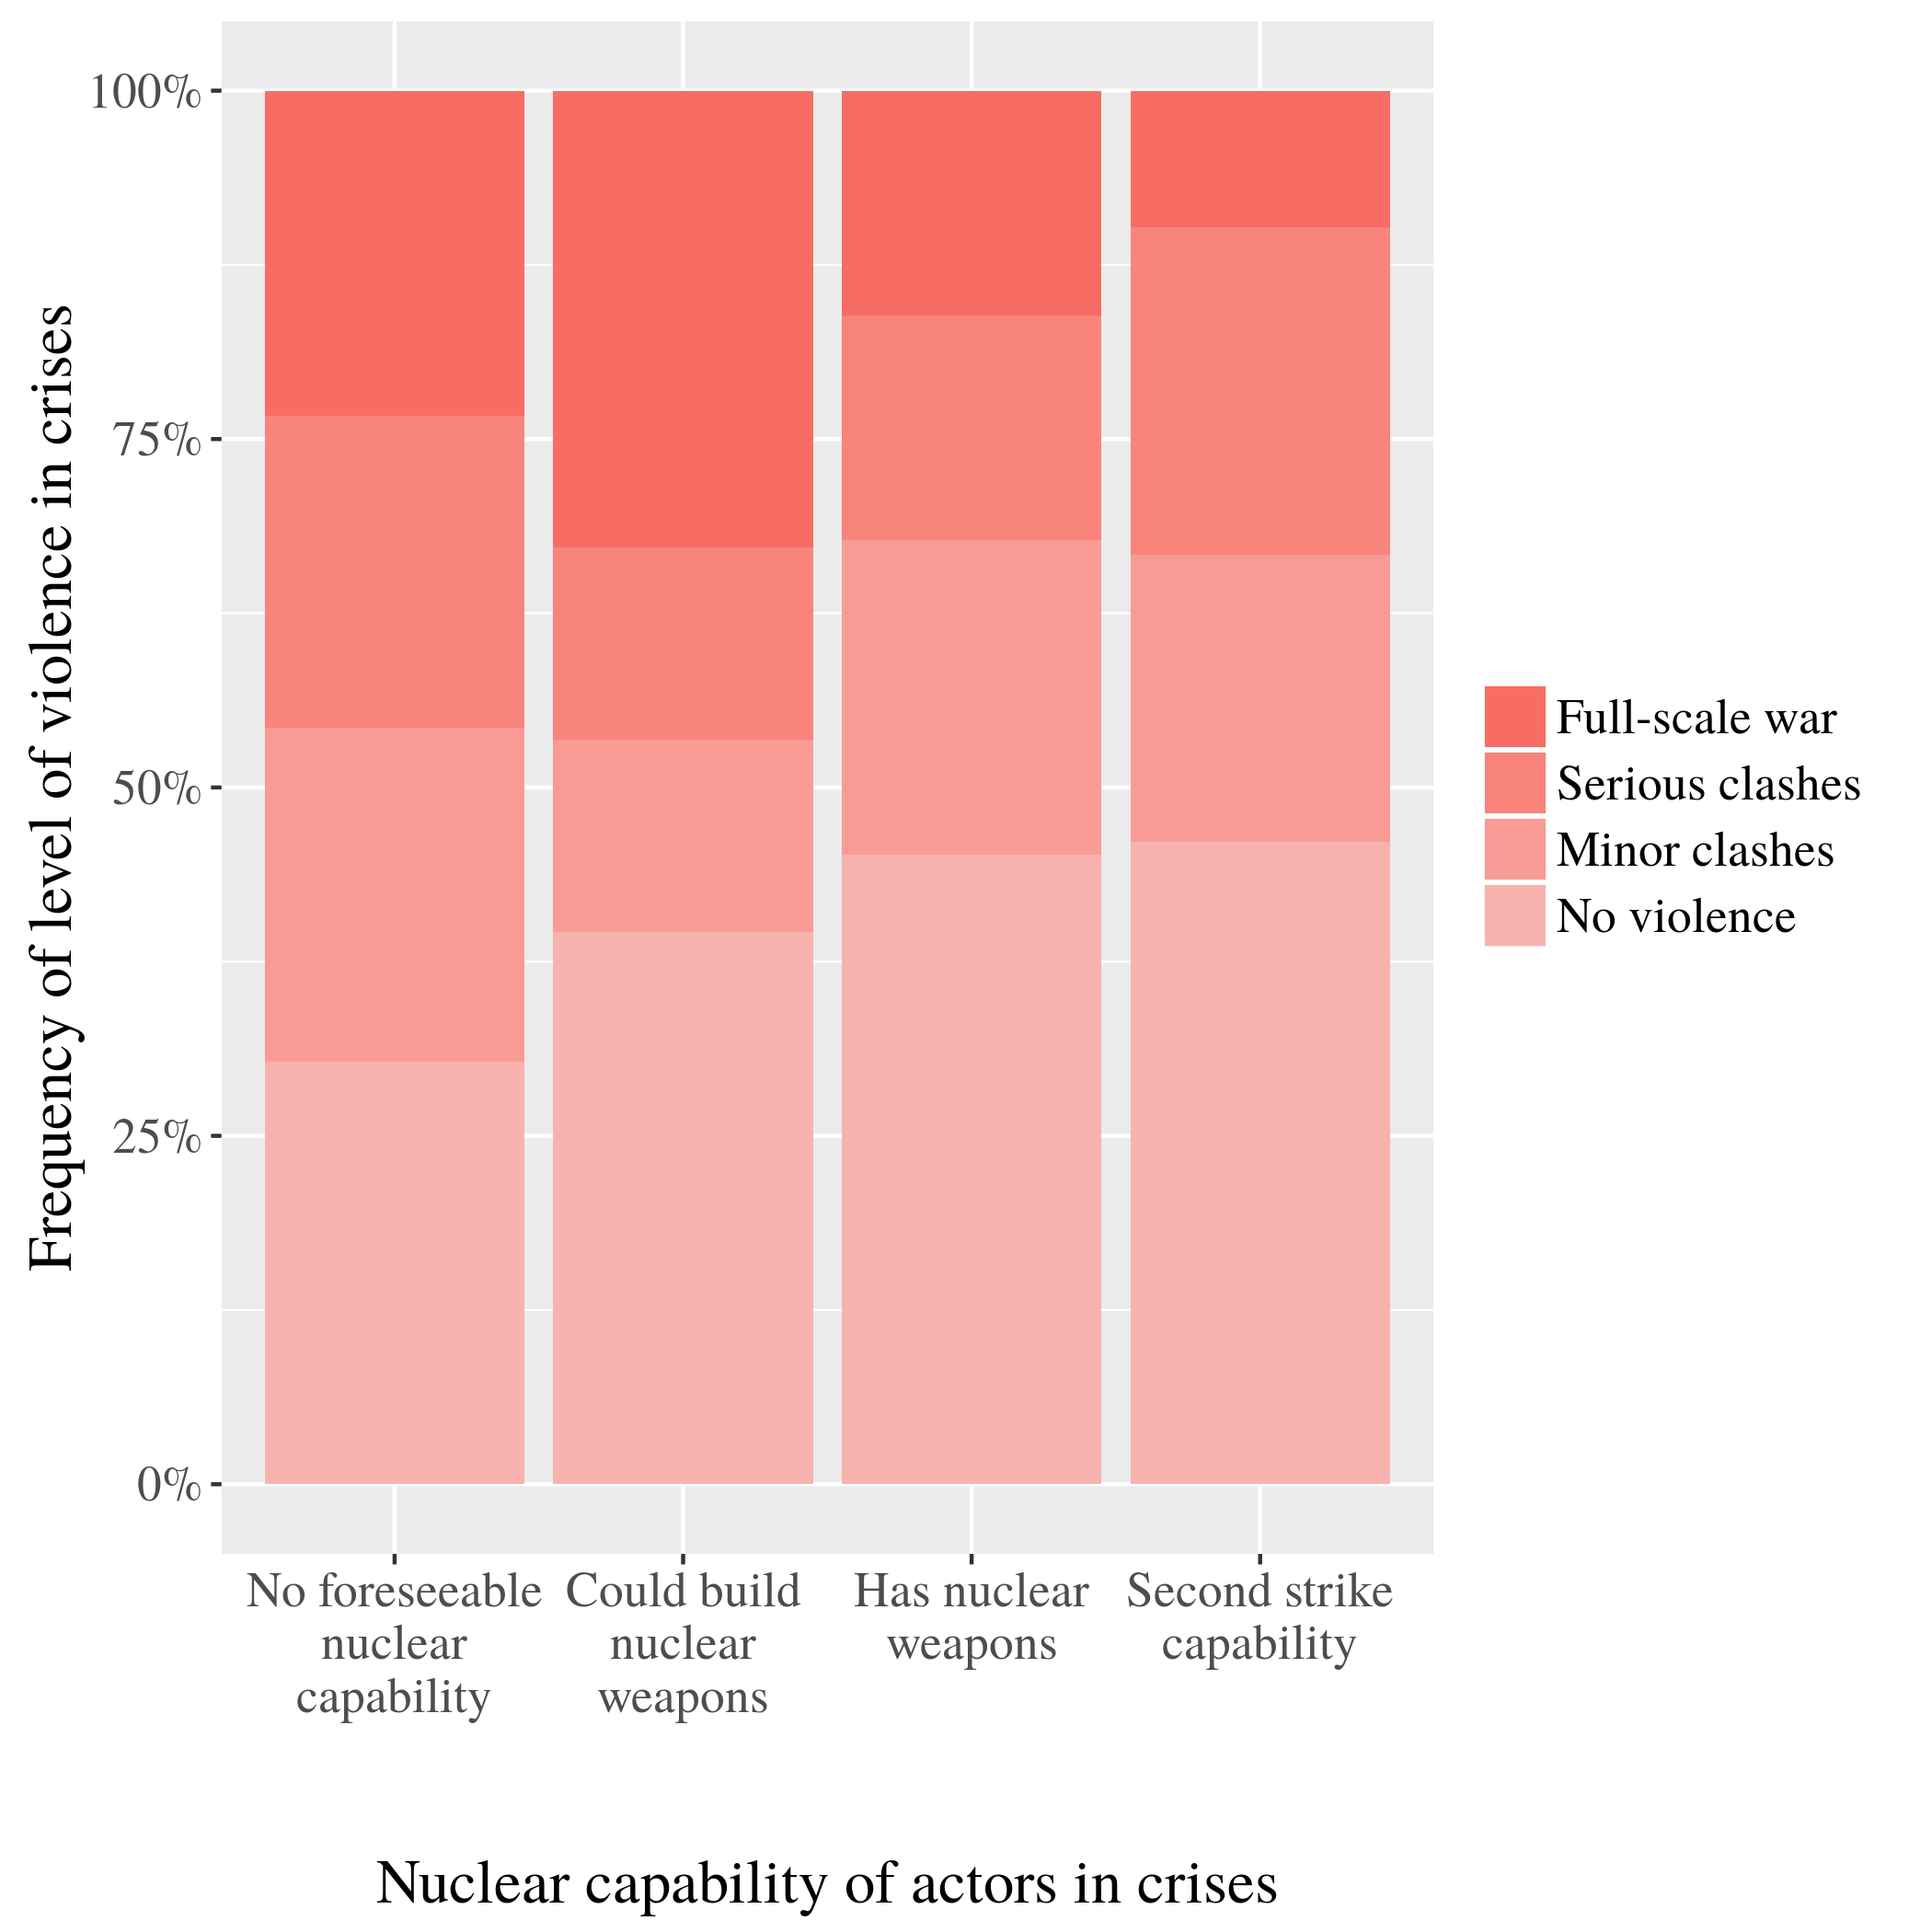
\includegraphics[width=\textwidth,height=0.47\textheight,keepaspectratio]{tmp/nuclear_compared_with_violence.pdf}
        \end{tabular}
    \end{table}
}

\end{document}
